\documentclass[dvipsnames,tikz]{standalone}
\usepackage{amsmath}
\usepackage{arevmath}
\usepackage{xcolor}
\usepackage{tikz}
\usetikzlibrary{calc}
\usetikzlibrary{decorations.pathreplacing,calligraphy,3d}
\usepackage{tikz-3dplot} 

\tikzset{main/.style={thick, circle, color=black}}

\newcommand{\arrowIn}{
	\tikz \draw[-stealth] (-1pt,0) -- (1pt,0);
}

\begin{document}
	
	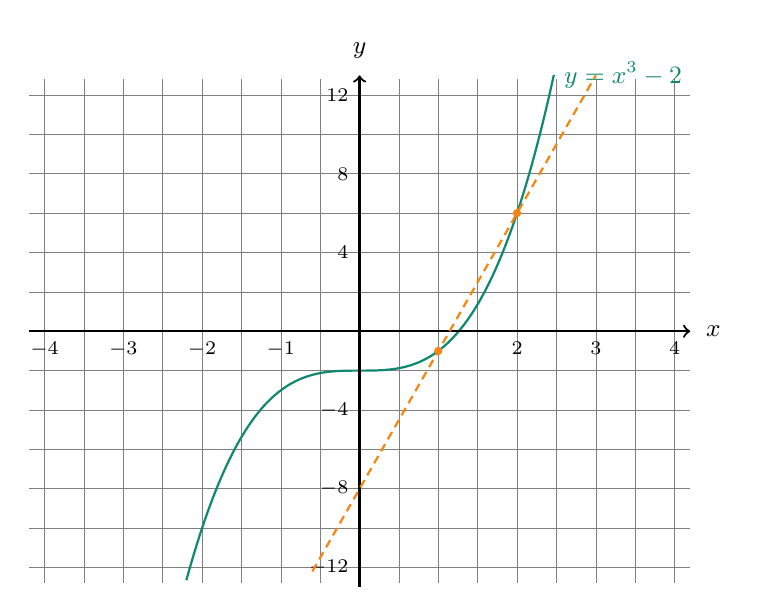
\begin{tikzpicture}[font=\small, tl/.style = {black, inner sep=1pt, font=\scriptsize} ]
		% grid
		\draw[main, very thin, xstep=0.5, ystep=0.5, semitransparent] (-4.2,-3.2) grid (4.2,3.2);
		
		% y tick label
		\foreach \y in {-12,-8,-4,4,8,12}{
			\node[tl,left=1mm] at (0,0.25*\y) {$\y$};
		}
		% x tick label
		\foreach \x in {-4,-3,-2,-1,2,3,4}{
			\node[tl,below=1mm] at (\x,0) {$\x$};
		}
		
		% curve
		\draw[thick,PineGreen,domain=-2.2:2.47,variable=\x, samples=200] plot(\x,{(\x*\x*\x-2)/4}) node [right] {$y=x^3-2$};
		
		% axes
		\draw[main, ->,thick] (-4.2,0) -- (4.2,0) node[right] {$x$};
		\draw[main, ->,thick] (0,-3.25) -- (0, 3.25) node[above] {$y$};	
		
		\fill[BurntOrange] (1,-0.25) circle (1.5pt);
		\fill[BurntOrange] (2,1.5) circle (1.5pt);
		\draw[thick, densely dashed,BurntOrange,domain=-0.6:3,variable=\x] plot(\x,7*\x/4-2);
	\end{tikzpicture}
	
	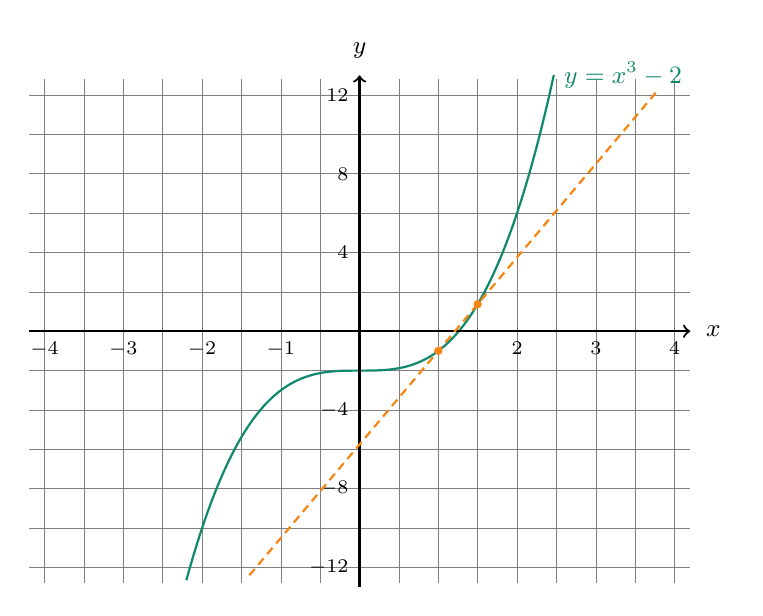
\begin{tikzpicture}[font=\small, tl/.style = {black, inner sep=1pt, font=\scriptsize} ]
		% grid
		\draw[main, very thin, xstep=0.5, ystep=0.5, semitransparent] (-4.2,-3.2) grid (4.2,3.2);
		
		% y tick label
		\foreach \y in {-12,-8,-4,4,8,12}{
			\node[tl,left=1mm] at (0,0.25*\y) {$\y$};
		}
		% x tick label
		\foreach \x in {-4,-3,-2,-1,2,3,4}{
			\node[tl,below=1mm] at (\x,0) {$\x$};
		}
		
		% curve
		\draw[thick,PineGreen,domain=-2.2:2.47,variable=\x, samples=200] plot(\x,{(\x*\x*\x-2)/4}) node [right] {$y=x^3-2$};
		
		% axes
		\draw[main, ->,thick] (-4.2,0) -- (4.2,0) node[right] {$x$};
		\draw[main, ->,thick] (0,-3.25) -- (0, 3.25) node[above] {$y$};	
		
		\fill[BurntOrange] (1,-0.25) circle (1.5pt);
		\fill[BurntOrange] (1.5,0.34375) circle (1.5pt);
		\draw[thick, densely dashed,BurntOrange,domain=-1.4:3.8,variable=\x] plot(\x, {(4.75*(\x-1)+1)/4-0.5});
	\end{tikzpicture}
	
	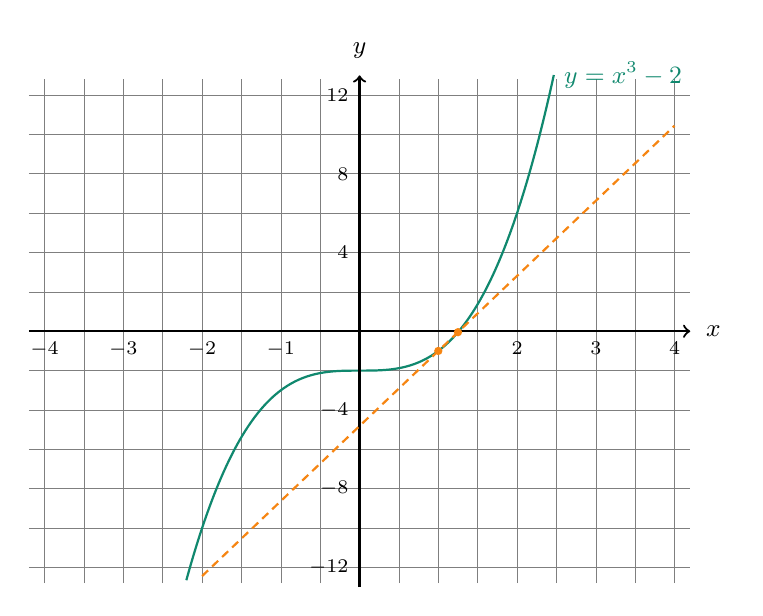
\begin{tikzpicture}[font=\small, tl/.style = {black, inner sep=1pt, font=\scriptsize} ]
		% grid
		\draw[main, very thin, xstep=0.5, ystep=0.5, semitransparent] (-4.2,-3.2) grid (4.2,3.2);
		
		% y tick label
		\foreach \y in {-12,-8,-4,4,8,12}{
			\node[tl,left=1mm] at (0,0.25*\y) {$\y$};
		}
		% x tick label
		\foreach \x in {-4,-3,-2,-1,2,3,4}{
			\node[tl,below=1mm] at (\x,0) {$\x$};
		}
		
		% curve
		\draw[thick,PineGreen,domain=-2.2:2.47,variable=\x, samples=200] plot(\x,{(\x*\x*\x-2)/4}) node [right] {$y=x^3-2$};
		
		% axes
		\draw[main, ->,thick] (-4.2,0) -- (4.2,0) node[right] {$x$};
		\draw[main, ->,thick] (0,-3.25) -- (0, 3.25) node[above] {$y$};	
		
		\fill[BurntOrange] (1,-0.25) circle (1.5pt);
		\fill[BurntOrange] (1.25,-.01171875) circle (1.5pt);
		\draw[thick, densely dashed,BurntOrange,domain=-2:4,variable=\x] plot(\x, {(3.8125*(\x-1)+1)/4-0.5});
	\end{tikzpicture}
	
	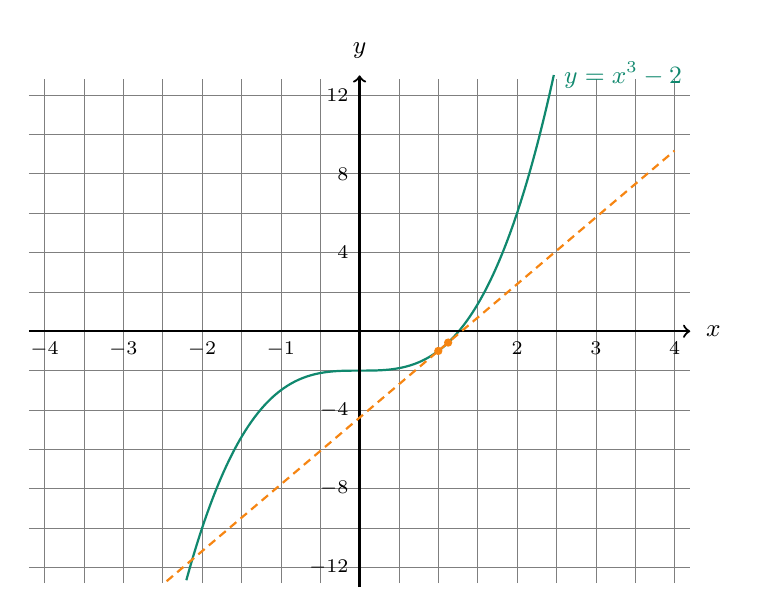
\begin{tikzpicture}[font=\small, tl/.style = {black, inner sep=1pt, font=\scriptsize} ]
		% grid
		\draw[main, very thin, xstep=0.5, ystep=0.5, semitransparent] (-4.2,-3.2) grid (4.2,3.2);
		
		% y tick label
		\foreach \y in {-12,-8,-4,4,8,12}{
			\node[tl,left=1mm] at (0,0.25*\y) {$\y$};
		}
		% x tick label
		\foreach \x in {-4,-3,-2,-1,2,3,4}{
			\node[tl,below=1mm] at (\x,0) {$\x$};
		}
		
		% curve
		\draw[thick,PineGreen,domain=-2.2:2.47,variable=\x, samples=200] plot(\x,{(\x*\x*\x-2)/4}) node [right] {$y=x^3-2$};
		
		% axes
		\draw[main, ->,thick] (-4.2,0) -- (4.2,0) node[right] {$x$};
		\draw[main, ->,thick] (0,-3.25) -- (0, 3.25) node[above] {$y$};	
		
		\fill[BurntOrange] (1,-0.25) circle (1.5pt);
		\fill[BurntOrange] (1.125,-.14404297) circle (1.5pt);
		\draw[thick, densely dashed,BurntOrange,domain=-2.45:4,variable=\x] plot(\x, {(3.390625*(\x-1)+1)/4-0.5});
	\end{tikzpicture}
	
	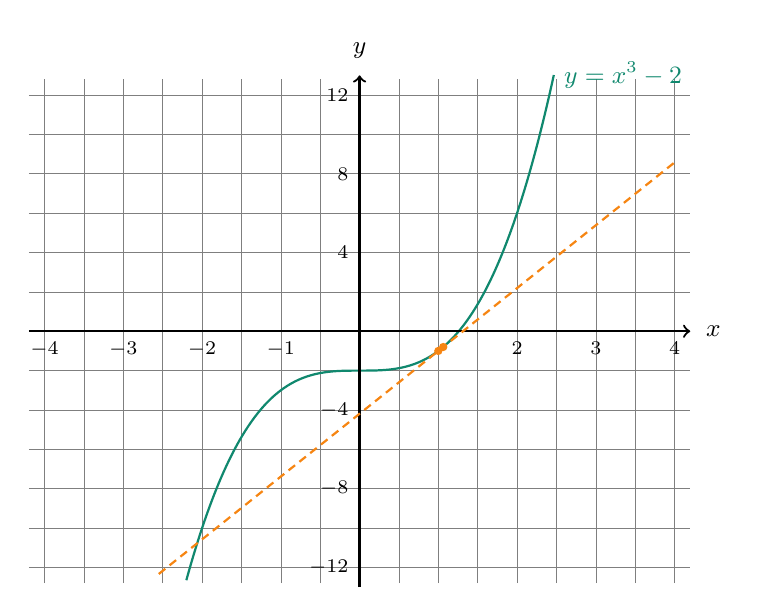
\begin{tikzpicture}[font=\small, tl/.style = {black, inner sep=1pt, font=\scriptsize} ]
		% grid
		\draw[main, very thin, xstep=0.5, ystep=0.5, semitransparent] (-4.2,-3.2) grid (4.2,3.2);
		
		% y tick label
		\foreach \y in {-12,-8,-4,4,8,12}{
			\node[tl,left=1mm] at (0,0.25*\y) {$\y$};
		}
		% x tick label
		\foreach \x in {-4,-3,-2,-1,2,3,4}{
			\node[tl,below=1mm] at (\x,0) {$\x$};
		}
		
		% curve
		\draw[thick,PineGreen,domain=-2.2:2.47,variable=\x, samples=200] plot(\x,{(\x*\x*\x-2)/4}) node [right] {$y=x^3-2$};
		
		% axes
		\draw[main, ->,thick] (-4.2,0) -- (4.2,0) node[right] {$x$};
		\draw[main, ->,thick] (0,-3.25) -- (0, 3.25) node[above] {$y$};	
		
		\fill[BurntOrange] (1,-0.25) circle (1.5pt);
		\fill[BurntOrange] (1+1/16,-.20013428) circle (1.5pt);
		\draw[thick, densely dashed,BurntOrange,domain=-2.55:4,variable=\x] plot(\x, {(3.19140625*(\x-1)+1)/4-0.5});
	\end{tikzpicture}
\end{document}